\documentclass[tikz,border=5pt]{standalone}
\usepackage{fontspec}
\setmainfont{Times New Roman}
\usepackage{unicode-math}
\setmathfont{Cambria Math}
\usetikzlibrary{shapes.geometric,positioning,fit,backgrounds,arrows.meta,calc}

\begin{document}
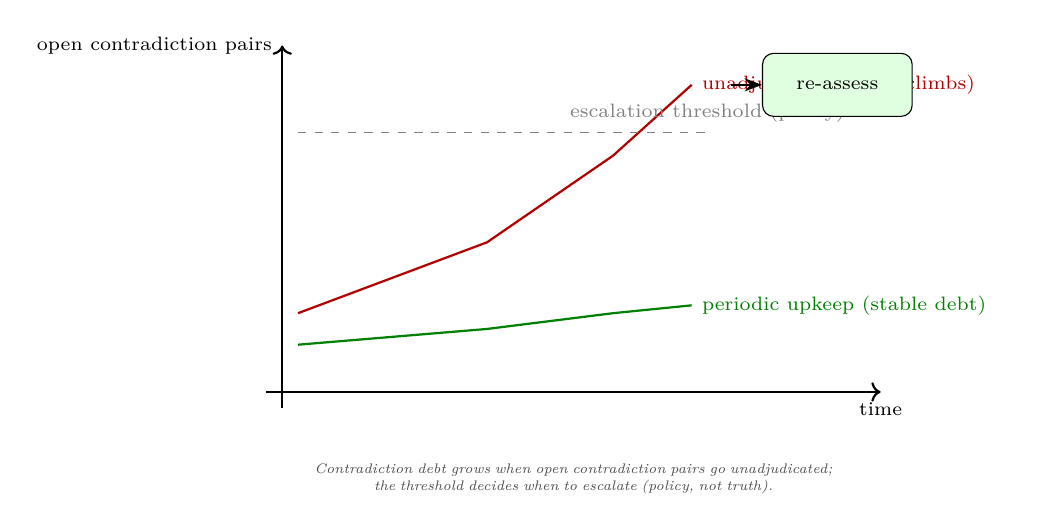
\begin{tikzpicture}[
  box/.style={rectangle, draw, rounded corners, align=center, font=\scriptsize, inner sep=3pt},
  arrow/.style={-{Stealth[length=2.2mm]}, thick},
  label/.style={font=\tiny\itshape, text=gray!60!black},
]

% === CONTRADICTION DEBT OVER TIME ===
\draw[->, thick] (-0.2, 0) -- (7.6, 0) node[below, font=\scriptsize] {time};
\draw[->, thick] (0, -0.2) -- (0, 4.4) node[left, font=\scriptsize] {open contradiction pairs};

\draw[thick, green!50!black] (0.2, 0.6) -- (2.6, 0.8) -- (4.2, 1.0) -- (5.2, 1.1) node[right, font=\scriptsize] {periodic upkeep (stable debt)};
\draw[thick, red!70!black] (0.2, 1.0) -- (2.6, 1.9) -- (4.2, 3.0) -- (5.2, 3.9) node[right, font=\scriptsize] {unadjudicated (debt climbs)};

\draw[dashed, gray] (0.2, 3.3) -- (5.4, 3.3) node[above, font=\scriptsize] {escalation threshold (policy)};

\node[box, fill=green!12, minimum width=1.9cm, minimum height=0.8cm] (actbox) at (7.05, 3.9) {re-assess};
\draw[arrow] (5.7, 3.9) -- (actbox);

\node[label, align=center, text width=11cm] at (3.7, -1.1)
  {Contradiction debt grows when open contradiction pairs go unadjudicated;\\the threshold decides when to escalate (policy, not truth).};
\end{tikzpicture}
\end{document}
